\documentclass{beamer}
\usepackage{kotex}
\usepackage{tikz}
\usepackage{graphicx}

\title{노트북에 Arch Linux 깔아서 써본 후기}
\author{신연진}

\begin{document}
\begin{frame}
    \maketitle
\end{frame}

\begin{frame}{목차}
    \tableofcontents
\end{frame}

\begin{frame}{기존의 노트북}
    \section{기존의 노트북}
    \begin{itemize}
     \item 노트북에 우분투와 윈도우를 설치해서 듀얼부팅으로 이용하고 있었음.
     \item 주변에 아치리눅스로 밀어버리고 쓰고 있는 친구가 있었는데, 그 친구를 보니 문득 아치 리눅스를 한 번 써보고 싶어졌다.
    \end{itemize}
\end{frame}

\begin{frame}{Arch linux란?}
    \section{Arch Liniux란?}
    \includegraphics[width=15em]{archlinux logo.png}
    \begin{itemize}
        \item x86/64 시스템에서 작동하는 가벼운 GNU/Linux 배포판
        \item 최초 설치시에는 ``최소한''만 깔리며 나머지는 사용자가 직접 취향에 맞게 설치해야 한다.
        \item GNOME/KDE등 DE가 기본으로 같이 설치되는 Ubuntu/Debian/RedHat 등 기존의 배포판과 달리, 리눅스를 밑바닥부터 자신의 취향대로 선택할 수 있다는 것이 장점.
        \item 문서화(위키)가 매우 잘 되어 있다.
    \end{itemize}
\end{frame}

\begin{frame}{롤링 릴리즈}
    \subsection{롤링 릴리즈?}
    \begin{itemize}
        \item Arch Linux는 Ubuntu와는 달리 롤링 릴리즈(Rolling Release, a.k.a. Continous Delivery) 방식을 채택한다.

        우분투처럼 릴리즈 버전(20.04, 22.02 등)이 붙지 않으며, 패키지 매니저의 업데이트 명령어를 실행하면 패키지들이 항상 최신 버전으로 업데이트된다. (우분투의 \texttt{do-release-upgrade} 명령어가 없는 느낌?)
    \end{itemize}
\end{frame}

\begin{frame}{롤링 릴리즈}
    \begin{figure}
        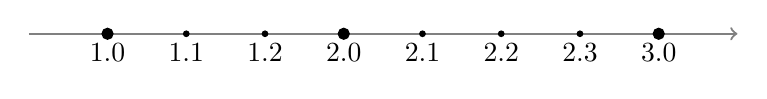
\begin{tikzpicture}
            \draw[gray, thick, ->] (-1,0) -- (8,0);
            \filldraw[black] (0,0) circle (2pt) node[anchor=north]{1.0};
            \filldraw[black] (1,0) circle (1pt) node[anchor=north]{1.1};
            \filldraw[black] (2,0) circle (1pt) node[anchor=north]{1.2};
            \filldraw[black] (3,0) circle (2pt) node[anchor=north]{2.0};
            \filldraw[black] (4,0) circle (1pt) node[anchor=north]{2.1};
            \filldraw[black] (5,0) circle (1pt) node[anchor=north]{2.2};
            \filldraw[black] (6,0) circle (1pt) node[anchor=north]{2.3};
            \filldraw[black] (7,0) circle (2pt) node[anchor=north]{3.0};
        \end{tikzpicture}
        \caption{우분투의 Point-release 방식}
    \end{figure}

    \begin{figure}
        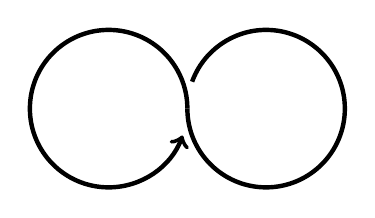
\begin{tikzpicture}
            \draw[ultra thick, ->] (0,0) arc (0:340:1);
            \draw[ultra thick] (0,0) arc (180:520:1);
        \end{tikzpicture}
        \caption{아치리눅스의 Rolling Release 방식}
    \end{figure}
\end{frame}

\begin{frame}{Pacman과 AUR}
    \subsection{Pacman과 AUR}
    \texttt{Pacman}은 Arch Linux의 패키지 매니저이다. (우분투의 \texttt{apt}, 데비안의 \texttt{rpm}과 비슷한 역할)
    \begin{itemize}
        \item 설치: \texttt{sudo pacman -S something}
        \item 삭제: \texttt{sudo pacman -Rs something}
        \item 시스템 전체 업그레이드: \texttt{sudo pacman -Syu}
        \item 안쓰는 의존성 삭제: \texttt{sudo pacman -R \$(sudo pacman -Qdtq)}
    \end{itemize}

    AUR은 이용자들이 유지보수하는 패키지들이 업로드되는 저장소이다.
    \begin{itemize}
     \item AUR에서 Git clone하고 (e.g. \texttt{https://git.archlinux.org/zoom.git}) 그 디렉토리 내에서 \texttt{makepkg -sic} 명령어 실행해서 설치하면 된다.
     \item \texttt{yay}처럼 AUR을 지원하는 패키지 매니저를 쓰기도 함.
    \end{itemize}

\end{frame}


\begin{frame}{설치}
    \section{설치}
    Arch Linux의 설치 CD/DVD(USB)는 꽂고 부팅하면 콘솔이 나타난다.
    \begin{figure}
        \includegraphics[scale=0.25]{archlinux iso boot.png}
        \caption{Arch Linux CD/DVD(USB)를 넣고 부팅한 모습}
    \end{figure}
    무언가 잘못된 것인가? $ \rightarrow $ 아님, 정상임. 이제 여기서 명령어를 입력하면서 설치하면 된다.
    자세한 방법은 아치리눅스 위키 참고해야...
\end{frame}

\begin{frame}{제 시스템의 구성}
    \section{제 시스템의 구성}
    한줄요약: lemurs (로그인 매니저) + KDE Plasma (DE) + Firefox FE + Thunderbird + KDE 앱 몇개 + 스팀 + 게임

\end{frame}


\end{document}
